\documentclass[border=2pt]{standalone}
\usepackage[T1]{fontenc}\usepackage{mathptmx}
\usepackage{amsmath,amssymb}\usepackage{tikz}\usepackage{pgfplots}
\pgfplotsset{compat=1.18}
\usetikzlibrary{shapes.geometric, arrows.meta, positioning, calc}
\setlength{\columnwidth}{3.45in}
\newcommand{\Pfree}{P_{\mathrm{free}}}\newcommand{\dfree}{d_{\mathrm{free}}}\newcommand{\pos}{\mathrm{pos}}
\newcommand{\ind}{\mathbf{1}}\newcommand{\Lin}{\mathcal{L}}
\pgfplotsset{ieeeplot/.style={width=\columnwidth, height=5.4cm,
 tick label style={font=\footnotesize}, label style={font=\footnotesize},
 legend style={font=\footnotesize, draw=black!60, fill=white, fill opacity=0.9, text opacity=1},
 grid=both, grid style={line width=0.2pt, draw=black!15}, major grid style={line width=0.3pt, draw=black!25},
 every axis plot/.append style={line width=0.8pt, mark size=2.2pt}}}
\begin{document}
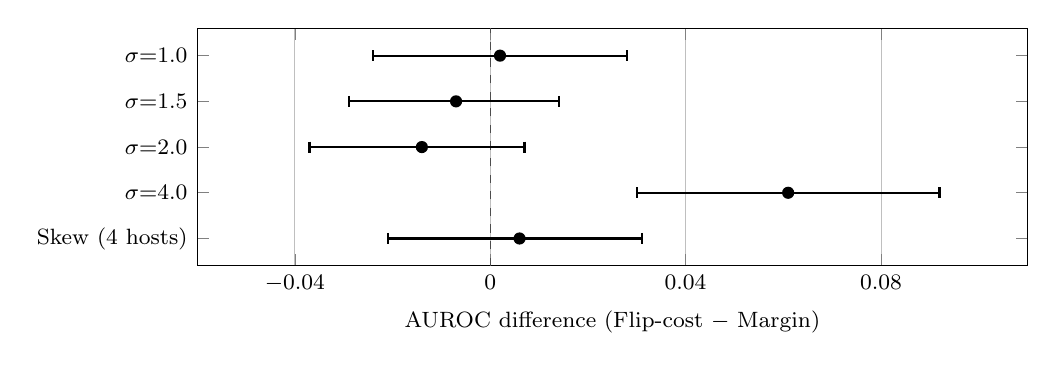
\begin{tikzpicture}
\begin{axis}[ieeeplot, height=4.6cm,
  xlabel={AUROC difference (Flip-cost $-$ Margin)}, xmin=-0.06, xmax=0.11,
  ymin=0.4, ymax=5.6, ytick={1,2,3,4,5},
  yticklabels={Skew (4 hosts), $\sigma{=}4.0$, $\sigma{=}2.0$, $\sigma{=}1.5$, $\sigma{=}1.0$},
  ymajorgrids=false, xtick={-0.04,0,0.04,0.08}, xticklabel style={/pgf/number format/fixed, /pgf/number format/precision=2}, scaled x ticks=false]
\draw[black!70, dashed] (axis cs:0,0.4) -- (axis cs:0,5.6);
\draw[thick] (axis cs:-0.024,5) -- (axis cs:0.028,5);
\draw[thick] (axis cs:-0.024,5.12) -- (axis cs:-0.024,4.88);
\draw[thick] (axis cs:0.028,5.12) -- (axis cs:0.028,4.88);
\fill (axis cs:0.002,5) circle (2.2pt);
\draw[thick] (axis cs:-0.029,4) -- (axis cs:0.014,4);
\draw[thick] (axis cs:-0.029,4.12) -- (axis cs:-0.029,3.88);
\draw[thick] (axis cs:0.014,4.12) -- (axis cs:0.014,3.88);
\fill (axis cs:-0.007,4) circle (2.2pt);
\draw[thick] (axis cs:-0.037,3) -- (axis cs:0.007,3);
\draw[thick] (axis cs:-0.037,3.12) -- (axis cs:-0.037,2.88);
\draw[thick] (axis cs:0.007,3.12) -- (axis cs:0.007,2.88);
\fill (axis cs:-0.014,3) circle (2.2pt);
\draw[thick] (axis cs:0.03,2) -- (axis cs:0.092,2);
\draw[thick] (axis cs:0.03,2.12) -- (axis cs:0.03,1.88);
\draw[thick] (axis cs:0.092,2.12) -- (axis cs:0.092,1.88);
\fill (axis cs:0.061,2) circle (2.2pt);
\draw[thick] (axis cs:-0.021,1) -- (axis cs:0.031,1);
\draw[thick] (axis cs:-0.021,1.12) -- (axis cs:-0.021,0.88);
\draw[thick] (axis cs:0.031,1.12) -- (axis cs:0.031,0.88);
\fill (axis cs:0.006,1) circle (2.2pt);
\end{axis}
\end{tikzpicture}
\end{document}
